\documentclass{beamer}

\mode<presentation>{
\usetheme{Madrid}
%\usecolortheme{beaver}
%\usecolortheme{crane}
}
\usepackage[utf8]{inputenc}
\usepackage{default}
\usepackage[portuguese]{babel}
\usepackage{pgfplots}
\pgfplotsset{/pgf/number format/use comma,compat=newest}
\usepackage{xcolor}
\usepackage{amsmath,amsfonts,amssymb}
\usepackage{hyperref}
\usepackage{tikz}

% \useoutertheme[subsection=false]{miniframes}

\definecolor{pene}{rgb}{.125,.4,.25}
\usecolortheme[named=pene]{structure}

%\usebackgroundtemplate{%
%\tikz\node[opacity=0.05] {\includegraphics[height=\paperheight,width=\paperwidth]{logoh_2.png}};}


\title[RECURRENT NEURAL NETWORKS WITH TOP-K GAINS  FOR SESSION-BASED RECOMMENDATIONS]{RECURRENT NEURAL NETWORKS WITH TOP-K GAINS  FOR SESSION-BASED RECOMMENDATIONS}
\subtitle{RNN Based Recommendation Engine}
\author{Muhammad Qasim \\ K191612@nu.edu.pk}
\institute[]{National University of Computer & Emerging Sciences}
\date{21 April 2021}

\begin{document}

\begin{frame}
 \maketitle
\end{frame}


\begin{frame}
\frametitle{13 Trillion Dollar}
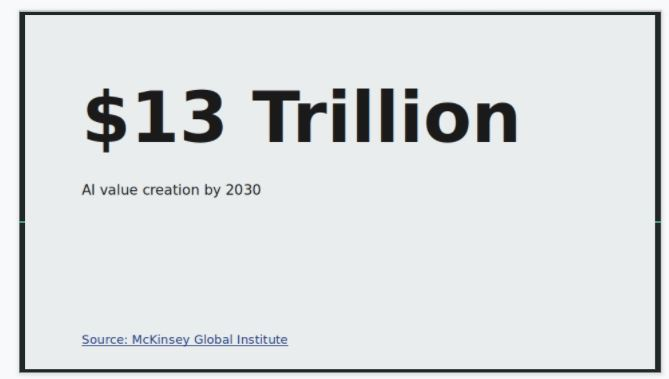
\includegraphics[width=\textwidth]{13 trillion.JPG}
\end{frame}


\begin{frame}
\frametitle{Industries Which create 13 Trillion dollar value}
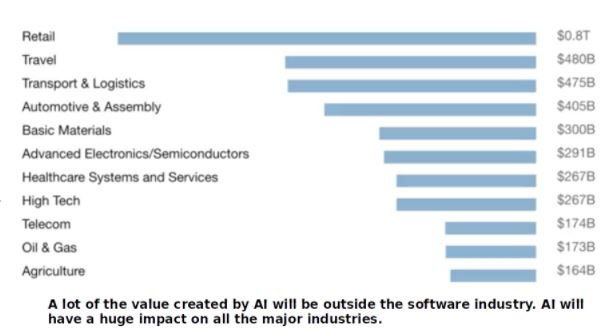
\includegraphics[width=\textwidth]{13 trillion_distribution.JPG}
\end{frame}


%\begin{frame}
%\frametitle{Contenido}
% \tableofcontents
%\end{frame}

\section{Recommendation Engine}
\begin{frame}
\frametitle{Recommendation Engine}
\begin{minipage}{\textwidth}
	\begin{itemize}
	\\~\\
    \item I have select this topic because i want to implement this research code for solving e-commerce platforms recommendation products and services. this recommendation engine will completely transform customers behaviour or it will be help to increase organizational profit. We know that RNN work perfectly on sequential data. So i will try to use \textbf{RNN} on customers login session transaction behaviour. It will recommend our products or service to our customers based on his/her previous purchasing behaviour. Author introduce a \textbf{novel ranking loss function tailored for RNNs in recom-mendation settings.} \\ \newline \newline
    \\~\\
    \item We improve results upto 35\% previous RNN session based recommendations in term of MPR and recall@20 and we also improve upto 51\% over classical collaborative filtering approaches. We didn’t use data augmentation technique to improve result. It’s save our training time.

    
    \end{itemize}

\end{minipage}
\end{frame}

\section{Key Features of paper}
\begin{frame}{Key Features of paper}
    \begin{columns}[t]
      \begin{column}{0.8\textwidth}
         \begin{block}{}
         
         \\~\\
             \begin{itemize}
              \item Suggest relevant products to users.(show top 3,5,10 or 20 items those user more likely)

              \item Ranking and loss function most important

              \item Pairwise ranking loss functions.
              \item Create new loss functions improve RNN performance up to 30\%
              
              \item We created loss and ranking function to improve up to 51\% over traditional collaborative filter recommendation



              \end{itemize}   
         \end{block}
      \end{column}
      
    \end{columns}
\end{frame} 


\begin{frame}
\frametitle{Research Questions}
\begin{minipage}{\textwidth}
	\begin{itemize}
    	\item Which algorithms will we be used?
    	\begin{itemize}
    	\item RNN, LSTM and collaborative filtering
    	\end{itemize}
    	
    	\item From Where you will get dataset?
    	\begin{itemize}
    	\item Movielens dataset
    	\end{itemize}
    	
    	\item Did you find some other technique?
    	\begin{itemize}
    	\item Collaborative filtering, user and item distance similarity matrix etc.
    	\end{itemize}
    	
    	\item Did you try to solve cold-start problem?
    	\begin{itemize}
    	\item Yes, technique provide good result to mitigate with this problem.
    	\end{itemize}
    	
    	\item How this research will help to business?
    	\begin{itemize}
    	\item It will totally transform any e-commerce based business.

    	\end{itemize}
    	
    	\item Are you satisfied with your work?
    	\begin{itemize}
    	\item 99\% satisfied with code base implementation 
    	\end{itemize}
    	
    	\item There are some other gap for new research?
    	\begin{itemize}
    	\item There are some areas where we can improve recommendation Engine.

    	\end{itemize}
    	
    	
      
    \end{itemize}
\end{minipage}
\end{frame} 

\begin{frame}{Technical Implementation Diagram}
    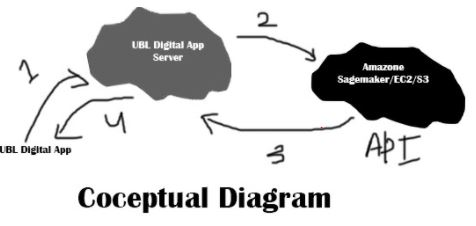
\includegraphics[width=\textwidth]{conceptual diagram.JPG}
\end{frame}

\begin{frame}{Research}
    \begin{itemize}
        \item RNN
        \item LSTM –Gated Recurrent Units (GRUs)Cho et al. (2014)
        \item RNN with Pairwise loss function(Tanet al., 2016)
        \item augmentation techniques (Hidasi et al., 2016b)
        \item loss functions tailored matrix factorization techniques (Weimer et al., 2007)

    \end{itemize}
\end{frame}


\begin{frame}{Literature Review}
\begin{itemize}
    \item Session based recommendation engine is such a good approach to recommend any product, based on user particular session time. Before session based recommendation engine we were using item based collaborative filtering (Sarwar et al., 2001)
    \item widely used linear product features transformation to memorization sparse matrices and Deep Learning low dimensional model for significant improvement on Google Play store app recommendation. (Heng-Tez Cheng et., 2020)
    \item use SVD to find the most relevant item to the new item. measured performance with Mean Absolute Error (MAE) and Root Mean Squared Error (RMSE) on realworld two datasets Movielens and Flixster dataset. It solved scalability, data sparsity and improvement of prediction and recommendation. (S.N. Gunjal et., 2020)
    \item RNN applied in speech recognition, translation, time series
    \item forecasting and signal processing. In recommender systems RNNs have been recently applied to the session-based recommendation setting with impressive results (Hidasi et al., 2016a)
\end{itemize}

\end{frame}


\begin{frame}
\frametitle{Research Gap}
\begin{minipage}{\textwidth}
	\begin{itemize}
    	\item We will try to combine RNN, LSTM and Some other Technique with together for better recommendation engine performance, or try to solve those problem we will facing previously machine learning algorithms.

	\end{itemize}
\end{minipage}
\end{frame} 

\begin{frame}
\frametitle{Research methodology }
	\begin{itemize}
    	\item I will select some major top journals, conferences for literature review.
    	
    	\begin{itemize}
    	    \item IEEE
    	    \item Elsevier
    	    \item AAAS
    	    \item WILEY
    	    \item ACM Computing Surveys
    	    \item Springer

    	\end{itemize}
    \end{itemize}
    
    
\end{frame} 





\begin{frame}
\frametitle{Technical contribution flowchart}
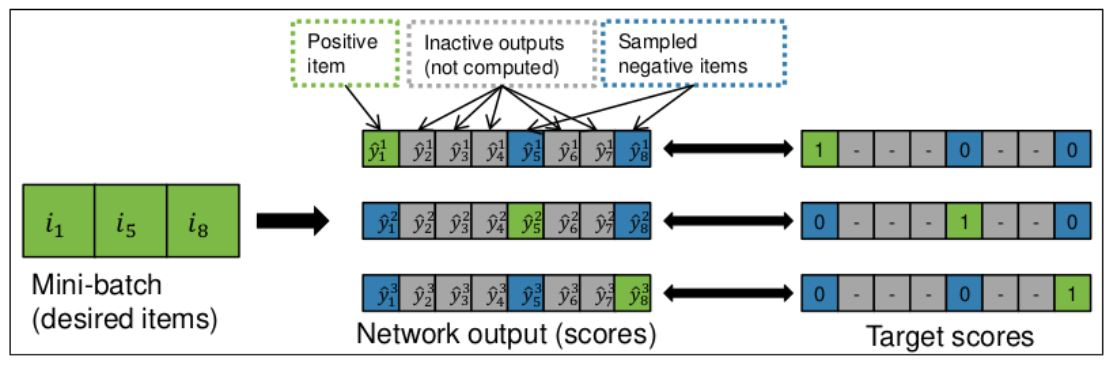
\includegraphics[width=\textwidth]{technical.JPG}	 
\end{frame} 

\begin{frame}{Conclusion}
    We improve results upto 35\% previous RNN session based recommendations in term of MPR and recall@20 and we also improve upto 51\% over classical collaborative filtering approaches. We didn’t use data augmentation technique to improve result. It’s save our training time.

\end{frame}

\begin{frame}{future direction}
    It is also conceivable that these techniques could also provide similar benefits in the area of Natural Language Processing a domain that shares significant similarities to the recommendation domain in terms of machine learning

\end{frame}

\begin{frame}
\begin{center}
    Thank You!
\end{center}
\end{frame} 

\end{document}
